% Provenance (never printed): see sources/outline_sources.md (Year 2: Goldschmidt's
% classification; the chondritic Earth; core, mantle and crust compositions; trace
% elements and normalised diagrams). Curves from figdata/bachelor-2/geochem.py; exercise
% and problem values in the Book 4 scratch calculator calc/ch03.py.
\chapter{पृथ्वी में तत्त्व}\label{ch:b2:elements-in-the-earth}

महाद्वीपों की एक टन चट्टान में लगभग डेढ़ मिलीग्राम सोना होता है। पिछले
अध्याय के \omterm{def:b2:planet-formation-meteorites:chondrule}{कार्बनमय कॉन्ड्राइटों} की, जो आकाश से गिरने वाले सबसे आदिम पत्थर हैं,
एक टन मात्रा में लगभग सौ गुना अधिक सोना होता है। पृथ्वी ऐसी ही सामग्री से
बनी, इसलिए सोना पृथ्वी से गायब नहीं है: वह कहीं और है। क्रोड और
सिलिकेट पृथ्वी के अनुमानित संघटनों को क्रोड के द्रव्यमान के साथ मिलाइए, तो पता चलता है कि
पृथ्वी का 99 प्रतिशत से अधिक सोना क्रोड में है, जहाँ वह पृथ्वी के इतिहास के
आरंभ में लोहे के साथ डूब गया। सोना उन तत्त्वों के एक परिवार का सदस्य है जो धात्विक
लोहे का अनुसरण करते हैं; अन्य सल्फ़ाइड का, अन्य
सिलिकेट चट्टान का अनुसरण करते हैं, और कुछ अन्य
वायु में निकल जाते हैं। यह अध्याय तत्त्वों को इन परिवारों में बाँटता है,
\omterm{def:b2:planet-formation-meteorites:chondrule}{कॉन्ड्राइटों} से पूरी पृथ्वी का संघटन पुनर्निर्मित करता है और उसके क्रोड को तौलता है,
प्रावार, महासागरीय भूपर्पटी और महाद्वीपीय भूपर्पटी के संघटनों का वर्णन करता है, और
\omterm{def:b2:elements-in-the-earth:trace}{अनुरेखी तत्त्वों} तथा उन आरेखों से परिचय कराता है जिन पर भू-रसायनविद्
किसी चट्टान का इतिहास पढ़ते हैं।
% ledger: rg03:ucc-trace, lodders:ci-table, mcd03:core, ms95:pm-trace, data:prem

\begin{recall}
पृथ्वी का एक धात्विक क्रोड है, मुख्यतः लोहे का, जिसके ऊपर सिलिकेट प्रावार और पतली
भूपर्पटी है; भूकंपविज्ञान हर परत की त्रिज्या और घनत्व देता है, और क्रोड
उसी दाब और तापमान पर शुद्ध लोहे की तुलना में 5 से 10 प्रतिशत कम घना है,
जो उसमें हल्के तत्त्वों की माँग करता है: सिलिकॉन, सल्फ़र, कार्बन,
ऑक्सीजन और हाइड्रोजन उम्मीदवार हैं (पुस्तक 3, स्नातक वर्ष 1)। किसी तत्त्व की
विद्युत्-ऋणात्मकता मापती है कि उसके परमाणु किसी आबंध के इलेक्ट्रॉनों को कितनी प्रबलता से
आकर्षित करते हैं, और किसी आयन की त्रिज्या उसके आवेश और उसके पड़ोसियों की संख्या पर
निर्भर करती है (रसायन-विज्ञान की पुस्तकें, प्रथम वर्ष)। विभाजन
गुणांक साम्यावस्था में दो प्रावस्थाओं में किसी पदार्थ की सांद्रताओं का
अनुपात है (रसायन-विज्ञान की पुस्तकें, प्रथम वर्ष)। \omterm{def:b2:planet-formation-meteorites:chondrule}{कॉन्ड्राइट}, \omterm{def:b2:planet-formation-meteorites:chondrule}{कार्बनमय
कॉन्ड्राइट} और \omterm{def:b2:planet-formation-meteorites:condensation}{संघनन अनुक्रम}
\cref{ch:b2:planet-formation-meteorites} में प्रस्तुत किए गए थे।
\end{recall}
% ledger: badro:core

\section{गोल्डश्मिट का वर्गीकरण}

जब कोई कॉन्ड्राइटी पिंड पिघलता है, तो उसका पदार्थ अमिश्रणीय द्रवों में पृथक हो जाता है:
लोहे और निकल की एक घनी धातु, पर्याप्त सल्फ़र हो तो एक सल्फ़ाइड द्रव, और एक
सिलिकेट गलित, जिसके ऊपर एक गैस प्रावस्था होती है। हर तत्त्व अपने रसायन के अनुसार
इन प्रावस्थाओं के बीच बँट जाता है, और यही विभाजन धातु-प्रगलन में दिखता है,
जहाँ भट्टी में पिघला लोहा, एक सल्फ़ाइड मैट और एक सिलिकेट धातुमल अलग हो
जाते हैं।

\begin{definition}[गोल्डश्मिट वर्गीकरण]
\label{def:b2:elements-in-the-earth:goldschmidt}
\emph{गोल्डश्मिट वर्गीकरण}\index{गोल्डश्मिट वर्गीकरण} तत्त्वों को
उस प्रावस्था के अनुसार छाँटता है जिसे वे धातु, सल्फ़ाइड, सिलिकेट और गैस में पृथक होने वाले पिंड में
पसंद करते हैं। \emph{शिलारागी तत्त्व}\index{शिलारागी तत्त्व}
सिलिकेट और ऑक्साइड को पसंद करता है; \emph{लौहरागी तत्त्व}\index{लौहरागी तत्त्व}
धात्विक लोहे को पसंद करता है; \emph{ताम्ररागी
तत्त्व}\index{ताम्ररागी तत्त्व} सल्फ़ाइड को पसंद करता है; \emph{वायुरागी
तत्त्व}\index{वायुरागी तत्त्व} गैस में रहता है, गैस या किसी वाष्पशील
यौगिक के रूप में।
\end{definition}

ये वर्ग आबंधन के रसायन का अनुसरण करते हैं। \omterm{def:b2:elements-in-the-earth:goldschmidt}{शिलारागी तत्त्व}, जैसे
क्षार और क्षारीय-मृदा धातुएँ, ऐलुमिनियम, टाइटेनियम या दुर्लभ मृदाएँ, अपने
इलेक्ट्रॉन सहजता से ऑक्सीजन को दे देते हैं, जो कहीं अधिक विद्युत्-ऋणात्मक है, और
उसके साथ आयनिक आबंध बनाते हैं। \omterm{def:b2:elements-in-the-earth:goldschmidt}{लौहरागी तत्त्व}, प्लैटिनम-समूह की धातुएँ, सोना,
निकल और कोबाल्ट, लोहे के निकट विद्युत्-ऋणात्मकता रखते हैं, ऑक्सीजन के साथ दुर्बल आबंध
बनाते हैं और धातु में घुल जाते हैं। \omterm{def:b2:elements-in-the-earth:goldschmidt}{ताम्ररागी तत्त्व}, जिनमें ताँबा, जस्ता, सीसा,
चाँदी और कैडमियम हैं, सल्फ़र के साथ अधिक सहसंयोजी आबंध बनाते हैं।
\omterm{def:b2:elements-in-the-earth:goldschmidt}{वायुरागी तत्त्व} उत्कृष्ट गैसें, नाइट्रोजन और हाइड्रोजन हैं। अनेक
तत्त्व परिस्थितियों के अनुसार दो वर्गों के होते हैं: स्वयं लोहा
धातु-समृद्ध पिंड में लौहरागी है और ऑक्सीकृत प्रावार में शिलारागी, जहाँ वह
ओलिवीन और पाइरॉक्सीन में रहता है; टंगस्टन और मॉलिब्डेनम पृथ्वी में लौहरागी हैं,
पर उनका बड़ा भाग प्रावार में रह गया (नीचे का चित्र)।

\begin{omfigure}
\centering
\begin{tikzpicture}[x=0.62cm, y=-0.62cm,
  lith/.style={fill=brown!30}, sid/.style={fill=blue!30!gray!45},
  chal/.style={fill=orange!45}, atm/.style={fill=cyan!15}, none/.style={fill=black!8},
  cell/.style={draw=black!55, minimum size=0.58cm, inner sep=0pt, font=\scriptsize}]
\foreach \s/\c/\r/\k in {H/1/1/atm, He/18/1/atm,
  Li/1/2/lith, Be/2/2/lith, B/13/2/lith, C/14/2/atm, N/15/2/atm, O/16/2/lith,
  F/17/2/lith, Ne/18/2/atm,
  Na/1/3/lith, Mg/2/3/lith, Al/13/3/lith, Si/14/3/lith, P/15/3/lith, S/16/3/chal,
  Cl/17/3/lith, Ar/18/3/atm,
  K/1/4/lith, Ca/2/4/lith, Sc/3/4/lith, Ti/4/4/lith, V/5/4/lith, Cr/6/4/lith,
  Mn/7/4/lith, Fe/8/4/sid, Co/9/4/sid, Ni/10/4/sid, Cu/11/4/chal, Zn/12/4/chal,
  Ga/13/4/chal, Ge/14/4/sid, As/15/4/chal, Se/16/4/chal, Br/17/4/lith, Kr/18/4/atm,
  Rb/1/5/lith, Sr/2/5/lith, Y/3/5/lith, Zr/4/5/lith, Nb/5/5/lith, Mo/6/5/sid,
  Tc/7/5/none, Ru/8/5/sid, Rh/9/5/sid, Pd/10/5/sid, Ag/11/5/chal, Cd/12/5/chal,
  In/13/5/chal, Sn/14/5/chal, Sb/15/5/chal, Te/16/5/chal, I/17/5/lith, Xe/18/5/atm,
  Cs/1/6/lith, Ba/2/6/lith, Hf/4/6/lith, Ta/5/6/lith, W/6/6/sid, Re/7/6/sid,
  Os/8/6/sid, Ir/9/6/sid, Pt/10/6/sid, Au/11/6/sid, Hg/12/6/chal, Tl/13/6/chal,
  Pb/14/6/chal, Bi/15/6/chal, Po/16/6/none, At/17/6/none, Rn/18/6/none,
  La/3/8/lith, Ce/4/8/lith, Pr/5/8/lith, Nd/6/8/lith, Pm/7/8/none, Sm/8/8/lith,
  Eu/9/8/lith, Gd/10/8/lith, Tb/11/8/lith, Dy/12/8/lith, Ho/13/8/lith,
  Er/14/8/lith, Tm/15/8/lith, Yb/16/8/lith, Lu/17/8/lith,
  Th/4/9/lith, U/6/9/lith}
  \node[cell, \k] at (\c,\r) {\s};
\node[cell, lith, minimum width=0.58cm] at (3,6) {\tiny La--Lu};
\draw[black!50, -latex] (3,6.32) -- (3,7.65);
% legend
\foreach \k/\t/\x/\y in {lith/शिलारागी/3.6/1, sid/लौहरागी/3.6/2,
  chal/ताम्ररागी/3.6/3, atm/वायुरागी/7.8/1, none/{\shortstack[l]{कोई स्थायी\\समस्थानिक नहीं}}/7.8/2}
  \node[cell, \k, label={[font=\scriptsize]right:\t}] at (\x,\y) {};
\end{tikzpicture}
\par\smallskip{\small स्थायी तत्त्वों के, और थोरियम तथा यूरेनियम के, जिनके दीर्घजीवी समस्थानिक पृथ्वी के जन्म से बचे हुए हैं, गोल्डश्मिट वर्ग, उस वर्ग के अनुसार रंगे हुए
जो पृथ्वी में प्रबल है; दुर्लभ मृदा पंक्ति के तत्त्व
La--Lu बॉक्स में हैं। कई तत्त्व दो वर्गों के हैं: लोहा, निकल और कोबाल्ट ऑक्सीकृत प्रावार में
शिलारागी भी हैं; कार्बन लौहरागी भी है, फ़ॉस्फ़ोरस उल्कापिंडों में
लौहरागी।}
\end{omfigure}

\section{कॉन्ड्राइटी पृथ्वी}

कोई भी पूरी पृथ्वी का नमूना नहीं ले सकता: क्रोड पहुँच से बाहर है, और
प्रावार पृष्ठ तक केवल टुकड़ों में पहुँचता है। इसलिए समग्र पृथ्वी का संघटन
साक्ष्य के दो अंशों से बनाया जाता है: \omterm{def:b2:planet-formation-meteorites:fall-find}{उल्कापिंड}, जो उस
सामग्री के नमूने हैं जिससे ग्रह बने, और प्रावार की चट्टानें तथा उससे आने वाले
गलित।

\begin{definition}[CI कॉन्ड्राइट]\label{def:b2:elements-in-the-earth:ci}
\emph{CI कॉन्ड्राइट}\index{CI कॉन्ड्राइट} \omterm{def:b2:planet-formation-meteorites:chondrule}{कार्बनमय कॉन्ड्राइटों} के उस समूह का
सदस्य है जिसका नाम इवुना \omterm{def:b2:planet-formation-meteorites:fall-find}{उल्कापिंड} पर रखा गया है: काले, भुरभुरे पत्थर
जो लगभग पूरी तरह सूक्ष्म-कणिक आधात्री से बने हैं, जलयुक्त खनिजों और
कार्बन से समृद्ध, लगभग कॉन्ड्रयूल-रहित। हाइड्रोजन, कार्बन, नाइट्रोजन, ऑक्सीजन और
उत्कृष्ट गैसों को छोड़कर, उनका संघटन सभी ज्ञात पदार्थों में
सूर्य के प्रकाशमंडल के संघटन के सबसे निकट है; वे भू-रसायन का संदर्भ संघटन हैं।
\end{definition}

इस समूह में पाँच \omterm{def:b2:planet-formation-meteorites:fall-find}{उल्कापिंड} हैं, सभी \omterm{def:b2:planet-formation-meteorites:fall-find}{पतित उल्कापिंड}: अले (1806), ऑर्गुइल
(1864), टोंक (1911), इवुना (1938) और रेवेलस्टोक (1965); ऑर्गुइल सबसे बड़ा है,
चौदह किलोग्राम का। समूह के लिए अपनाया गया संघटन उनके विश्लेषणों का, तत्त्व-दर-तत्त्व,
भारित माध्य है; इस अध्याय में प्रयुक्त मान
जहाँ आवश्यक हैं वहीं उद्धृत किए गए हैं।
% ledger: lodders:ci-table

\begin{definition}[दुर्गलनीय और वाष्पशील तत्त्व]
\label{def:b2:elements-in-the-earth:volatility}
\emph{दुर्गलनीय तत्त्व}\index{दुर्गलनीय तत्त्व} वह है जिसका 50 प्रतिशत
\omterm{def:b2:planet-formation-meteorites:condensation}{संघनन तापमान} (\cref{ch:b2:planet-formation-meteorites})
मैग्नीशियम, सिलिकॉन और लोहे के \omterm{def:b2:planet-formation-meteorites:condensation}{संघनन तापमानों} से ऊपर है, जो \qty{e-4}{bar} पर \qtyrange{1310}{1340}{K}
हैं; \emph{वाष्पशील
तत्त्व}\index{वाष्पशील तत्त्व} वह है जिसका \omterm{def:b2:planet-formation-meteorites:condensation}{संघनन
तापमान} उनसे नीचे है।
\end{definition}

मैग्नीशियम की मात्रा मापदंड का काम करती है। मैग्नीशियम शिलारागी है, चट्टान के
मुख्य भाग के साथ संघनित होता है और क्रोड में प्रवेश नहीं करता, इसलिए सिलिकेट पृथ्वी में
किसी तत्त्व का मैग्नीशियम से अनुपात, \omterm{def:b2:elements-in-the-earth:ci}{CI कॉन्ड्राइटों} के उसी अनुपात से भाग देने पर,
मापता है कि कॉन्ड्राइटी आरंभिक सामग्री की तुलना में सिलिकेट पृथ्वी ने उस तत्त्व का कितना भाग
बनाए रखा। \omterm{def:b2:elements-in-the-earth:ci}{CI कॉन्ड्राइटों} में उपस्थित जल, कार्बन और अन्य वाष्पशील यौगिक, जिन्हें
पृथ्वी ने नहीं रखा, अनुपात से कट जाते हैं।

\begin{definition}[समग्र सिलिकेट पृथ्वी, आद्य प्रावार]
\label{def:b2:elements-in-the-earth:bse}
\emph{समग्र सिलिकेट पृथ्वी}\index{समग्र सिलिकेट पृथ्वी} क्रोड के बिना
पृथ्वी है: प्रावार, भूपर्पटी, महासागर और वायुमंडल एक साथ, जैसे वे
मिश्रित होने पर होते। इसी संघटन को \emph{आद्य प्रावार}\index{आद्य प्रावार}
कहते हैं: वह प्रावार जैसा वह क्रोड बनने के बाद और उससे कोई भूपर्पटी
निकाले जाने से पहले था।
\end{definition}

\omterm{def:b2:elements-in-the-earth:bse}{आद्य प्रावार} के अनुमान उन प्रावार चट्टानों पर टिके हैं जिन्होंने
सबसे कम गलित खोया है, अर्थात् लावाओं में ज़ेनोलिथ के रूप में ऊपर लाए गए (नीचे का फ़ोटो) या
पर्वत-पट्टियों में अनावृत पेरिडोटाइट, और इस मान्यता पर कि दुर्गलनीय \omterm{def:b2:elements-in-the-earth:goldschmidt}{शिलारागी
तत्त्व} एक-दूसरे के सापेक्ष कॉन्ड्राइटी अनुपातों में हैं। एक व्यापक रूप से प्रयुक्त परिणाम,
द्रव्यमान से 22.8 प्रतिशत मैग्नीशियम, 21.0 प्रतिशत सिलिकॉन और 6.26 प्रतिशत लोहे के साथ,
आगे संघटनों की तालिका में दिया गया है।
% ledger: ms95:pm-trace, ms95:pm-oxides

\begin{omfigure}
\centering
\begin{minipage}{0.48\linewidth}
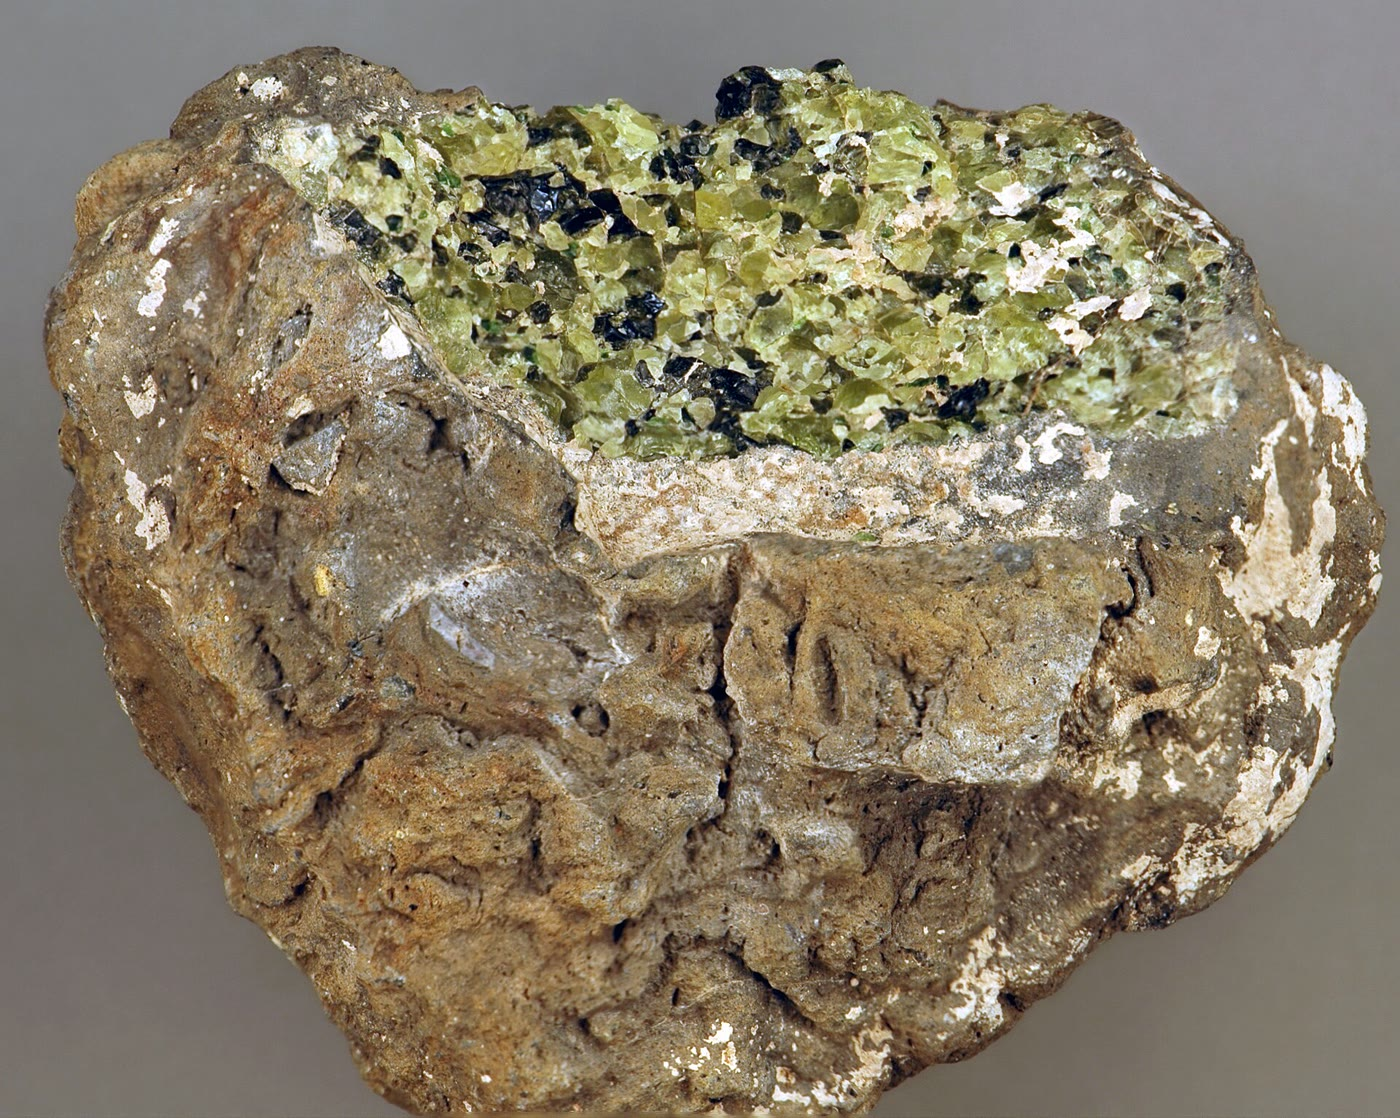
\includegraphics[width=\linewidth]{images/book4/b2-lherzolite-xenolith.jpg}
\end{minipage}\hfill
\begin{minipage}{0.48\linewidth}
{\small न्यू मेक्सिको के किलबोर्न होल के एक बेसाल्ट लावा में प्रावार पेरिडोटाइट (लर्ज़ोलाइट) की
एक गुटिका, अपने सबसे चौड़े भाग पर \qty{7.4}{cm}: पीला-हरा
ओलिवीन और गहरा पाइरॉक्सीन। लावा ने उसे ऊपरी प्रावार से तोड़ा और पृष्ठ तक
ले आया। फ़ोटो: James St.~John, CC BY 2.0।}
\end{minipage}
\end{omfigure}

नीचे का चित्र इस सिलिकेट पृथ्वी की तुलना \omterm{def:b2:elements-in-the-earth:ci}{CI कॉन्ड्राइटों} से, तत्त्व-दर-तत्त्व,
पिछले अध्याय के \omterm{def:b2:planet-formation-meteorites:condensation}{संघनन तापमान} के सापेक्ष करता है। यह तत्त्वों को
ऐसे छाँटता है जैसे कोई अन्य साक्ष्य नहीं कर सकता। दुर्गलनीय \omterm{def:b2:elements-in-the-earth:goldschmidt}{शिलारागी
तत्त्व}, ज़र्कोनियम और दुर्लभ मृदाओं से लेकर स्ट्रॉन्शियम और बेरियम तक, सभी
एक ही स्तर पर हैं, एक-दूसरे के बीस प्रतिशत के भीतर: सिलिकेट पृथ्वी ने
उन सबको उनके कॉन्ड्राइटी अनुपातों में रखा। वाष्पशील \omterm{def:b2:elements-in-the-earth:goldschmidt}{शिलारागी तत्त्व}
अपने \omterm{def:b2:planet-formation-meteorites:condensation}{संघनन तापमान} के साथ घटते जाते हैं: पोटैशियम और सोडियम का लगभग पाँचवाँ भाग,
रुबिडियम का दसवाँ भाग, क्लोरीन का सौवाँ भाग और ब्रोमीन तथा आयोडीन के कुछ
हज़ारवें भाग वहाँ हैं। \omterm{def:b2:elements-in-the-earth:goldschmidt}{लौहरागी तत्त्व} समान वाष्पशीलता के हर \omterm{def:b2:elements-in-the-earth:goldschmidt}{शिलारागी तत्त्व} से
बहुत नीचे हैं: सिलिकेट पृथ्वी में अपने हिस्से का लोहे का सातवाँ भाग,
निकल का तेरहवाँ भाग, और प्लैटिनम-समूह की धातुओं तथा सोने के लगभग तीन हज़ारवें भाग
हैं। ये क्रोड में चले गए। \omterm{def:b2:elements-in-the-earth:goldschmidt}{ताम्ररागी
तत्त्व}, जिनमें से अधिकांश वाष्पशील भी हैं, दोनों कारणों से न्यून हैं।

\begin{omfigure}
\centering
\begin{tikzpicture}
\begin{axis}[omrecord, width=0.95\linewidth, height=8.2cm, ymode=log,
  xmin=500, xmax=1800, ymin=8e-4, ymax=3, x dir=reverse,
  xlabel={\qty{e-4}{bar} पर 50 प्रतिशत संघनन तापमान (K)},
  ylabel={$(X/\mathrm{Mg})_{\mathrm{BSE}}\,/\,(X/\mathrm{Mg})_{\mathrm{CI}}$},
  legend pos=south west, legend cell align=left, legend style={font=\scriptsize},
  tick label style={font=\scriptsize}, label style={font=\small},
  scaled x ticks=false, xticklabel style={/pgf/number format/1000 sep={}}]
\addplot[black!40, dashed, domain=500:1800, samples=2, forget plot] {1};
\addplot[only marks, mark=*, mark size=1.6pt, brown!70!black]
  table[x=T, y=ratio] {figdata/out/bachelor-2-geochem-volat-lith.dat};
\addlegendentry{शिलारागी}
\addplot[only marks, mark=square*, mark size=1.6pt, blue!60!black]
  table[x=T, y=ratio] {figdata/out/bachelor-2-geochem-volat-sid.dat};
\addlegendentry{लौहरागी}
\addplot[only marks, mark=triangle*, mark size=2pt, orange!80!black]
  table[x=T, y=ratio] {figdata/out/bachelor-2-geochem-volat-chal.dat};
\addlegendentry{ताम्ररागी}
\node[font=\tiny, brown!50!black, anchor=south] at (axis cs:1600,1.35)
  {Zr, Hf, Al, Sc, Y, Th, U, Ti, Ca, Sr, Ba, दुर्लभ मृदाएँ};
\begin{scope}[font=\tiny, brown!50!black]
\node[anchor=west] at (axis cs:1328,1.0) {Mg};
\node[anchor=north] at (axis cs:1310,0.80) {Si};
\node[anchor=west] at (axis cs:1150,0.23) {Mn};
\node[anchor=south] at (axis cs:1142,0.47) {Li};
\node[anchor=south] at (axis cs:1010,0.195) {K};
\node[anchor=north] at (axis cs:958,0.22) {Na};
\node[anchor=north] at (axis cs:908,0.175) {B};
\node[anchor=north] at (axis cs:800,0.116) {Rb};
\node[anchor=south] at (axis cs:734,0.175) {F};
\node[anchor=west] at (axis cs:795,0.0477) {Cs};
\node[anchor=west] at (axis cs:944,0.0102) {Cl};
\node[anchor=north] at (axis cs:546,0.0061) {Br};
\node[anchor=south] at (axis cs:535,0.0088) {I};
\end{scope}
\begin{scope}[font=\tiny, blue!50!black]
\node[anchor=west] at (axis cs:1325,0.144) {Fe};
\node[anchor=east] at (axis cs:1364,0.0775) {Ni};
\node[anchor=west] at (axis cs:1342,0.088) {Co};
\node[anchor=west] at (axis cs:1780,0.137) {W};
\node[anchor=south] at (axis cs:1590,0.0206) {Mo};
\node[anchor=north] at (axis cs:883,0.0139) {Ge};
\node[anchor=north] at (axis cs:1500,0.0026) {Re, Os, Ir, Ru, Pt, Pd};
\node[anchor=north] at (axis cs:1060,0.0026) {Au};
\end{scope}
\begin{scope}[font=\tiny, orange!60!black]
\node[anchor=west] at (axis cs:1030,0.0993) {Cu};
\node[anchor=north] at (axis cs:996,0.0167) {Ag};
\node[anchor=south] at (axis cs:726,0.0746) {Zn};
\node[anchor=south] at (axis cs:704,0.0325) {Sn};
\node[anchor=east] at (axis cs:735,0.0246) {Pb};
\node[anchor=west] at (axis cs:648,0.0249) {Cd};
\node[anchor=east] at (axis cs:715,0.0022) {Te};
\node[anchor=north] at (axis cs:690,0.0016) {Se};
\node[anchor=west] at (axis cs:660,0.0019) {S};
\end{scope}
\end{axis}
\end{tikzpicture}
\par\smallskip{\small \omterm{def:b2:elements-in-the-earth:ci}{CI कॉन्ड्राइटों} की तुलना में सिलिकेट पृथ्वी: हर तत्त्व $X$ के लिए,
\omterm{def:b2:elements-in-the-earth:bse}{समग्र सिलिकेट पृथ्वी} में अनुपात $X/\mathrm{Mg}$, \omterm{def:b2:elements-in-the-earth:ci}{CI कॉन्ड्राइटों} के उसी अनुपात से
भाग देकर, 50 प्रतिशत \omterm{def:b2:planet-formation-meteorites:condensation}{संघनन तापमान} के सापेक्ष (गरम बाईं ओर)।
दुर्गलनीय \omterm{def:b2:elements-in-the-earth:goldschmidt}{शिलारागी तत्त्व} एक-दूसरे के सापेक्ष कॉन्ड्राइटी हैं; \omterm{def:b2:elements-in-the-earth:volatility}{वाष्पशील
तत्त्व} घटते \omterm{def:b2:planet-formation-meteorites:condensation}{संघनन तापमान} के साथ न्यून होते जाते हैं; लौहरागी और
\omterm{def:b2:elements-in-the-earth:goldschmidt}{ताम्ररागी तत्त्व} कहीं अधिक न्यून हैं। डेटा: McDonough और Sun (1995);
Lodders (2003)।}
\end{omfigure}
% ledger: ms95:pm-trace, lodders:ci-table, lodders:tc-table, lodders:tc-more

दुर्गलनीय \omterm{def:b2:elements-in-the-earth:goldschmidt}{शिलारागी तत्त्व} मैग्नीशियम से लगभग 15 प्रतिशत ऊपर हैं। दोनों
एक साथ ठीक-ठीक कॉन्ड्राइटी नहीं हो सकते: या तो पृथ्वी ने \omterm{def:b2:elements-in-the-earth:volatility}{दुर्गलनीय
तत्त्व} प्राप्त किए, या उसने थोड़ा मैग्नीशियम खोया, या मॉडल का मैग्नीशियम
कम आँका गया है (\cref{exo:b2:elements-in-the-earth:12})। सिलिकॉन, 0.83 पर, दुर्गलनीय स्तर से
और भी नीचे है; गायब सिलिकॉन का कुछ भाग क्रोड में हो सकता है (समस्या)।

सिलिकेट पृथ्वी के \omterm{def:b2:elements-in-the-earth:goldschmidt}{लौहरागी तत्त्व}, कॉन्ड्राइटी समग्र पृथ्वी के साथ मिलकर,
क्रोड को तौलते हैं। मान लीजिए समग्र पृथ्वी में CI अनुपात $r_X = X/\mathrm{Mg}$ है,
किसी \omterm{def:b2:elements-in-the-earth:goldschmidt}{लौहरागी तत्त्व} $X$ के लिए, और क्रोड में उसकी सांद्रता $c_X$ है
पर कोई मैग्नीशियम नहीं।

\begin{proposition}[कॉन्ड्राइटी अनुपात से क्रोड का द्रव्यमान-अंश]
\label{prop:b2:elements-in-the-earth:core}
मान लीजिए $x$ क्रोड का द्रव्यमान-अंश है, $C_X$ और $C_{\mathrm{Mg}}$
सिलिकेट पृथ्वी में $X$ और मैग्नीशियम की सांद्रताएँ हैं, और $c_X$
क्रोड में $X$ की सांद्रता। यदि पृथ्वी का कॉन्ड्राइटी अनुपात $r_X$ है, तो
\[
  \frac{x}{1-x} = \frac{r_X C_{\mathrm{Mg}} - C_X}{c_X}.
\]
\end{proposition}

\begin{proof}
पृथ्वी के $M$ द्रव्यमान में $(1-x)MC_X + xMc_X$ मात्रा $X$ की और $(1-x)MC_{\mathrm{Mg}}$
मात्रा मैग्नीशियम की होती है। इनका अनुपात $r_X$ है:
$(1-x)C_X + xc_X = r_X(1-x)C_{\mathrm{Mg}}$। $(1-x)c_X$ से भाग देने पर
परिणाम मिलता है।
\end{proof}

लोहे के साथ, \omterm{def:b2:elements-in-the-earth:ci}{CI कॉन्ड्राइटों} में $r_{\mathrm{Fe}} = \num{182800}/\num{95870} = 1.907$,
सिलिकेट पृथ्वी में 22.8 प्रतिशत मैग्नीशियम और 6.26 प्रतिशत लोहा, और एक मॉडल क्रोड में 85.5
प्रतिशत लोहा लेने पर, प्रतिज्ञप्ति $x/(1-x) = 0.435$ देती है, अर्थात् पृथ्वी के द्रव्यमान का 30
प्रतिशत क्रोड। भूकंपविज्ञान, संदर्भ पृथ्वी मॉडल के घनत्व का समाकलन करके,
32.5 प्रतिशत देता है। दसवें भाग के भीतर यह सहमति
उस कॉन्ड्राइटी पृथ्वी के चित्र का समर्थन करती है जिसका लोहा अधिकतर क्रोड में है;
अंतर मापता है कि पृथ्वी का लोहा-से-मैग्नीशियम अनुपात कॉन्ड्राइटी अनुपात से कितना
हटता है (समस्या)। यही संतुलन बताता है कि पृथ्वी का हर तत्त्व कहाँ है
(नीचे का चित्र): उसका लगभग सारा प्लैटिनम, इरिडियम और सोना, और उसके लोहे,
निकल और सल्फ़र का अधिकांश, क्रोड में है।
% ledger: lodders:ci-table, ms95:pm-trace, mcd03:core, data:prem

\begin{omfigure}
\centering
\begin{tikzpicture}
\begin{axis}[omrecord, xbar, width=0.8\linewidth, height=6.4cm, bar width=5pt,
  xmin=0, xmax=100, ymin=0.4, ymax=14.6, y dir=reverse,
  ytick={1,...,14}, yticklabels from table={figdata/out/bachelor-2-geochem-budget.dat}{el},
  xlabel={पृथ्वी की कुल मात्रा का क्रोड में स्थित अंश (प्रतिशत)},
  tick label style={font=\scriptsize}, label style={font=\small},
  nodes near coords, nodes near coords align={horizontal},
  every node near coord/.append style={font=\tiny, /pgf/number format/fixed,
    /pgf/number format/precision=1}]
\addplot[fill=blue!35!gray!50, draw=black!60]
  table[x=share, y=idx] {figdata/out/bachelor-2-geochem-budget.dat};
\end{axis}
\end{tikzpicture}
\par\smallskip{\small पृथ्वी के तत्त्व कहाँ हैं: हर तत्त्व का वह अंश जो
क्रोड में है, एक मॉडल क्रोड-संघटन, \omterm{def:b2:elements-in-the-earth:bse}{आद्य प्रावार} और पृथ्वी के द्रव्यमान के 32.5
प्रतिशत क्रोड से। डेटा: McDonough (2003); McDonough और Sun (1995);
संदर्भ पृथ्वी मॉडल।}
\end{omfigure}
% ledger: mcd03:core, ms95:pm-trace, data:prem

\section{प्रावार और भूपर्पटियाँ}

सिलिकेट पृथ्वी अपने निर्माण से ही एक प्रावार और दो
प्रकार की भूपर्पटी में बँटी हुई है। महासागरीय भूपर्पटी मध्य-महासागरीय कटकों के नीचे प्रावार के
गलन से बनती है; महाद्वीपीय भूपर्पटी क्षेपण क्षेत्रों के ऊपर गलन, पुनर्संसाधन और
अपरदन के लंबे इतिहास से (आगे के अध्याय)। प्रावार के दो संदर्भ गलित
चर्चा को आधार देते हैं।

\begin{definition}[मध्य-महासागरीय कटक बेसाल्ट, महासागरीय द्वीप बेसाल्ट]
\label{def:b2:elements-in-the-earth:morb-oib}
\emph{मध्य-महासागरीय कटक बेसाल्ट}\index{मध्य-महासागरीय कटक बेसाल्ट} (MORB) वह बेसाल्ट है
जो किसी मध्य-महासागरीय कटक पर उद्गारित हुआ, महासागरीय भूपर्पटी के शीर्ष की चट्टान।
\emph{महासागरीय द्वीप बेसाल्ट}\index{महासागरीय द्वीप बेसाल्ट} (OIB) वह बेसाल्ट है जो
प्लेट-सीमाओं से दूर किसी महासागरीय ज्वालामुखी पर उद्गारित हुआ, जैसे हवाई के ज्वालामुखी,
और जिसे सामान्यतः किसी प्रावार-स्तंभ से जोड़ा जाता है (पुस्तक 3, स्नातक वर्ष 1)।
\end{definition}

नीचे की तालिका का माध्य MORB 771 कटक-खंडों से बना एक वैश्विक औसत है,
जिसमें हर खंड को उसकी लंबाई और उसकी विस्तारण-दर से भारित किया गया है, ताकि
औसत उस भूपर्पटी का प्रतिनिधित्व करे जो कटक बनाते हैं। OIB
स्तंभ एक ही चट्टान है: बेसाल्ट संदर्भ पदार्थ BHVO-2, जो 1995 में
उस लावा से लिया गया जो 1919 में हवाई के किलाउआ के हालेमाउमाउ गर्त से उमड़ा था,
और जिसका विश्लेषण अनेक प्रयोगशालाओं ने किया, ताकि उसकी अधिकांश दुर्लभ मृदाएँ
लगभग एक प्रतिशत तक ज्ञात हैं। ऊपरी महाद्वीपीय भूपर्पटी पृष्ठ की चट्टानों और अवसादों से
अनुमानित एक औसत है।
% ledger: gale13:allmorb, usgs:bhvo2-origin, usgs:bhvo2-major, rg14:crust

\begin{table}[h]
\centering
\small
\begin{tabular}{lrrrr}
\hline
ऑक्साइड (भार\,\%) & \omterm{def:b2:elements-in-the-earth:bse}{आद्य प्रावार} & MORB & OIB (BHVO-2) & ऊपरी महाद्वीपीय भूपर्पटी\\
\hline
\ce{SiO2} & 45.0 & 50.47 & 49.60 & 66.6\\
\ce{TiO2} & 0.201 & 1.68 & 2.731 & 0.64\\
\ce{Al2O3} & 4.45 & 14.70 & 13.44 & 15.4\\
FeO (कुल) & 8.05 & 10.43 & 11.15 & 5.04\\
MnO & 0.135 & 0.184 & 0.1690 & 0.10\\
MgO & 37.8 & 7.58 & 7.257 & 2.48\\
CaO & 3.55 & 11.39 & 11.40 & 3.59\\
\ce{Na2O} & 0.36 & 2.79 & 2.219 & 3.27\\
\ce{K2O} & 0.029 & 0.160 & 0.5130 & 2.80\\
\ce{P2O5} & 0.021 & 0.184 & 0.2685 & 0.15\\
\hline
\end{tabular}
\caption{चार भंडारों के मुख्य-तत्त्व संघटन। BHVO-2 अपना लोहा
\ce{Fe2O3} (12.39 प्रतिशत) के रूप में देता है, जिसे यहाँ FeO में बदला गया है।
डेटा: McDonough और Sun (1995); Gale और अन्य (2013); BHVO-2 के लिए USGS
सूचना-पत्रक; Rudnick और Gao (2014)।}
\label{tab:b2:elements-in-the-earth:majors}
\end{table}
% ledger: ms95:pm-oxides, gale13:allmorb, usgs:bhvo2-major, rg14:crust

पंक्ति-दर-पंक्ति पढ़ने पर तालिका गलन की कहानी कहती है। प्रावार एक मैग्नीशियम-समृद्ध
पेरिडोटाइट है, लगभग 38 प्रतिशत MgO और 5 प्रतिशत से कम \ce{Al2O3} और CaO।
इसके गलितों, बेसाल्टों, में पाँच गुना कम मैग्नीशियम और तीन गुना अधिक
कैल्सियम और ऐलुमिनियम है: जो तत्त्व सहजता से गलित में प्रवेश करते हैं वे प्रावार को
पहले छोड़ते हैं। पोटैशियम, सोडियम और टाइटेनियम प्रावार की तुलना में गलितों में और भी
समृद्ध हैं, और पोटैशियम महाद्वीपीय भूपर्पटी में सबसे अधिक समृद्ध है,
\omterm{def:b2:elements-in-the-earth:bse}{आद्य प्रावार} में अपनी सांद्रता का लगभग सौ गुना। सिलिकॉन प्रावार से बेसाल्टों तक
केवल थोड़ा बढ़ता है, और महाद्वीपीय भूपर्पटी में कहीं अधिक, जिसका
औसत ग्रैनोडायोराइट के निकट है।

\section{अनुरेखी तत्त्व}

ऊपर की तालिका की हर चट्टान का लगभग 99 प्रतिशत दस ऑक्साइड बनाते हैं। शेष तत्त्व,
जो प्रति मिलियन भागों में उपस्थित हैं, मुख्य तत्त्वों जैसी ही प्रक्रियाओं का अनुसरण करते हैं, पर
वे उनके प्रति कहीं अधिक संवेदनशील हैं।

\begin{definition}[अनुरेखी तत्त्व]\label{def:b2:elements-in-the-earth:trace}
किसी चट्टान का \emph{अनुरेखी तत्त्व}\index{अनुरेखी तत्त्व} वह तत्त्व है जिसकी
सांद्रता परिपाटी के अनुसार द्रव्यमान से 0.1 प्रतिशत (\qty{1000}{ppm}) से कम है।
अनुरेखी तत्त्व विरले ही अपने स्वयं के खनिज बनाते हैं; वे क्रिस्टल-जालकों के स्थलों में मुख्य
तत्त्वों को प्रतिस्थापित करते हैं।
\end{definition}

\omterm{def:b2:elements-in-the-earth:trace}{अनुरेखी तत्त्व} इतना तनु होता है कि उसकी अपनी सांद्रता क्रिस्टलों या
गलित को नहीं बदलती: तब उनके बीच उसका वितरण एक सरल अनुपात होता है,
जो एक विस्तृत परास में उसकी सांद्रता से स्वतंत्र है।

\begin{definition}[खनिज--गलित विभाजन गुणांक; संगत और
असंगत तत्त्व]\label{def:b2:elements-in-the-earth:partition}
किसी खनिज में किसी तत्त्व का \emph{खनिज--गलित विभाजन गुणांक}\index{खनिज--गलित विभाजन गुणांक}
खनिज में और उसके साथ साम्यावस्था में स्थित सिलिकेट गलित में उसकी सांद्रताओं का
अनुपात है,
$D = C_{\mathrm{mineral}}/C_{\mathrm{melt}}$। कई खनिजों वाली चट्टान के लिए, जिनके
द्रव्यमान-अंश $x_i$ हैं, \emph{समग्र विभाजन गुणांक}
$\bar D = C_{\mathrm{rock}}/C_{\mathrm{melt}}$ है। कोई तत्त्व किसी चट्टान में
\emph{संगत तत्त्व}\index{संगत तत्त्व} है यदि $\bar D > 1$,
और \emph{असंगत तत्त्व}\index{असंगत तत्त्व} यदि $\bar D < 1$।
\end{definition}

\begin{proposition}[समग्र विभाजन गुणांक]
\label{prop:b2:elements-in-the-earth:bulk-d}
यदि चट्टान का हर खनिज एक ही गलित के साथ साम्यावस्था में है, तो समग्र
विभाजन गुणांक खनिज-गुणांकों का द्रव्यमान-अंशों से भारित
औसत है: $\bar D = \sum_i x_i D_i$।
\end{proposition}

\begin{proof}
चट्टान में $C_{\mathrm{rock}} = \sum_i x_i C_i$ है, और हर खनिज में
$C_i = D_i C_{\mathrm{melt}}$। $C_{\mathrm{melt}}$ से भाग देने पर परिणाम मिलता है।
\end{proof}

कोई आयन किसी स्थल में समाता है या नहीं, यह उसकी त्रिज्या और उसके आवेश पर निर्भर करता है। जो आयन
त्रिज्या और आवेश में स्थल के मुख्य आयन के निकट हो, जैसे \ce{Ni^2+}, जो ओलिवीन में
\ce{Mg^2+} का स्थान लेता है, वह आसानी से प्रवेश करता है और संगत है। बहुत बड़ा आयन, जैसे
\ce{Rb+} या \ce{Ba^2+}, या अधिक आवेशित आयन, जैसे \ce{Zr^4+} या
\ce{Nb^5+}, जालक पर तनाव डालता है और गलित में अस्वीकृत हो जाता है: वह
प्रावार के खनिजों में असंगत है। \omterm{def:b2:elements-in-the-earth:partition}{असंगत तत्त्वों} के दो समूह
आगे चलकर, जब जल सम्मिलित होता है, भिन्न व्यवहार करते हैं।

\begin{definition}[बृहत्-आयन शिलारागी और उच्च क्षेत्र-सामर्थ्य तत्त्व]
\label{def:b2:elements-in-the-earth:lile-hfse}
\emph{बृहत्-आयन शिलारागी तत्त्व}\index{बृहत्-आयन शिलारागी तत्त्व}
(LILE) बड़े, कम आवेश वाले, $+1$ या $+2$, आयनों वाले \omterm{def:b2:elements-in-the-earth:partition}{असंगत तत्त्व} हैं:
पोटैशियम, रुबिडियम, सीज़ियम, स्ट्रॉन्शियम, बेरियम।
\emph{उच्च क्षेत्र-सामर्थ्य तत्त्व}\index{उच्च क्षेत्र-सामर्थ्य तत्त्व} (HFSE)
छोटे, उच्च आवेश वाले, $+4$ या $+5$, आयनों वाले \omterm{def:b2:elements-in-the-earth:partition}{असंगत तत्त्व} हैं:
ज़र्कोनियम, हैफ़नियम, नायोबियम, टैंटलम, टाइटेनियम।
\end{definition}

LILE जल-समृद्ध तरलों में आसानी से घुलते हैं, HFSE लगभग बिल्कुल नहीं। जल से
परिवर्तित चट्टान या तरल विरासत में पाने वाला गलित, जैसे क्षेपण क्षेत्रों के ऊपर,
इसलिए कम HFSE के साथ LILE लिए होता है।

\begin{definition}[दुर्लभ मृदा तत्त्व]\label{def:b2:elements-in-the-earth:ree}
\emph{दुर्लभ मृदा तत्त्व}\index{दुर्लभ मृदा तत्त्व} (REE) पंद्रह
लैंथेनाइड हैं, लैंथेनम से ल्यूटेशियम तक; प्रोमेथियम का कोई स्थायी समस्थानिक नहीं है। सभी
शिलारागी और दुर्गलनीय हैं, लगभग सभी त्रिसंयोजी, और उनकी आयनिक त्रिज्या
लैंथेनम से ल्यूटेशियम तक लगातार घटती है; अपचयित गलितों में यूरोपियम
द्विसंयोजी भी हो सकता है।
\end{definition}

चूँकि दुर्लभ मृदाएँ केवल त्रिज्या में, और वह भी सुचारु रूप से, भिन्न हैं, वे
सुचारु रूप से प्रभाजित होती हैं: हल्की, लैंथेनम से सैमेरियम तक, सबसे कम
संगत हैं; भारी, गैडोलिनियम से ल्यूटेशियम तक, कुछ खनिजों में बेहतर समाती हैं,
सबसे अधिक गार्नेट में (नीचे का चित्र)। गार्नेट वाली चट्टान में भारी दुर्लभ
मृदाएँ संगत हो जाती हैं: ऐसी चट्टान का गलित हल्की दुर्लभ मृदाओं में समृद्ध और
भारी में निर्धन होता है।

\begin{omfigure}
\centering
\begin{tikzpicture}
\begin{axis}[omrecord, width=0.78\linewidth, height=6.4cm, ymode=log,
  xmin=0.6, xmax=9.4, ymin=5e-4, ymax=20,
  xtick={1,...,9}, xticklabels from table={figdata/out/bachelor-2-geochem-dvals.dat}{el},
  ylabel={विभाजन गुणांक $D$}, legend pos=south east,
  legend cell align=left, legend style={font=\scriptsize},
  tick label style={font=\scriptsize}, label style={font=\small}]
\addplot[black!40, dashed, domain=0.6:9.4, samples=2, forget plot] {1};
\addplot[thick, green!45!black, mark=*] table[x=idx, y=cpx] {figdata/out/bachelor-2-geochem-dvals.dat};
\addlegendentry{क्लाइनोपाइरॉक्सीन}
\addplot[thick, red!70!black, mark=square*] table[x=idx, y=gar] {figdata/out/bachelor-2-geochem-dvals.dat};
\addlegendentry{गार्नेट}
\addplot[thick, olive!70!black, mark=triangle*] table[x=idx, y=ol] {figdata/out/bachelor-2-geochem-dvals.dat};
\addlegendentry{ओलिवीन + ऑर्थोपाइरॉक्सीन + स्पिनेल}
\addplot[very thick, black, mark=diamond*] table[x=idx, y=bulk] {figdata/out/bachelor-2-geochem-dvals.dat};
\addlegendentry{समग्र चट्टान (65/18/17 प्रतिशत)}
\node[font=\scriptsize, anchor=south west] at (axis cs:0.7,1) {संगत};
\node[font=\scriptsize, anchor=north west] at (axis cs:0.7,1) {असंगत};
\end{axis}
\end{tikzpicture}
\par\smallskip{\small क्लाइनोपाइरॉक्सीन, गार्नेट और ओलिवीन, ऑर्थोपाइरॉक्सीन तथा स्पिनेल के एक मिश्रण के लिए
दुर्लभ मृदाओं के \omterm{def:b2:elements-in-the-earth:partition}{खनिज--गलित विभाजन गुणांक}, और 65 प्रतिशत क्लाइनोपाइरॉक्सीन, 18 प्रतिशत
गार्नेट और 17 प्रतिशत अन्य खनिजों वाले गार्नेट पाइरॉक्सिनाइट का समग्र
गुणांक (ऊपर की प्रतिज्ञप्ति)। गार्नेट
भारी दुर्लभ मृदाओं को संगत बनाता है। डेटा: Budahn (1991)।}
\end{omfigure}
% ledger: budahn91:d-ree, budahn91:modes

\section{प्रसामान्यीकृत आरेख}

पड़ोसी तत्त्वों की प्रचुरताएँ पदार्थ के नाभिकीय इतिहास के कारण बड़े गुणकों से भिन्न होती हैं:
सम परमाणु-क्रमांक वाले तत्त्व अपने विषम पड़ोसियों से अधिक प्रचुर हैं,
जैसा दुर्लभ मृदाओं का CI स्तंभ दिखाता है (लैंथेनम 0.232,
सीरियम 0.621, प्रेसियोडिमियम 0.0928 ppm)। कच्चे रूप में आलेखित करने पर किसी चट्टान की दुर्लभ मृदाएँ
एक आरा-दाँत बनाती हैं जो उसके भूवैज्ञानिक इतिहास को छिपा देता है। किसी संदर्भ से भाग देने पर यह हट जाता है।
% ledger: lodders:ci-table

\begin{definition}[प्रसामान्यीकृत आरेख]\label{def:b2:elements-in-the-earth:normalised}
\emph{प्रसामान्यीकृत आरेख}\index{प्रसामान्यीकृत आरेख} तत्त्वों की किसी
नियत क्रम वाली शृंखला के लिए, किसी नमूने में सांद्रता को किसी संदर्भ की सांद्रता से
भाग देकर, $X_N = C_X/C_X^{\mathrm{ref}}$, लघुगणकीय पैमाने पर आलेखित करता है। दुर्लभ मृदाएँ
परमाणु-क्रमांक के क्रम में \omterm{def:b2:elements-in-the-earth:ci}{CI कॉन्ड्राइटों} से प्रसामान्यीकृत की जाती हैं; \omterm{def:b2:elements-in-the-earth:partition}{असंगत तत्त्वों} का
एक लंबा समुच्चय, जिसे प्रायः मकड़ी आरेख कहते हैं, \omterm{def:b2:elements-in-the-earth:bse}{आद्य प्रावार} से प्रसामान्यीकृत होता है
और प्रावार-गलन में घटती असंगतता के क्रम में रखा जाता है।
\end{definition}

संदर्भ जैसे ही अनुपातों वाला नमूना एक क्षैतिज रेखा के रूप में आलेखित होता है;
उसकी ऊँचाई समृद्धि देती है। ढलान हल्के और भारी तत्त्वों के बीच
प्रभाजन दिखाती है, जिसे $(\mathrm{La}/\mathrm{Yb})_N$ जैसे अनुपात से मापा जाता है।
रेखा से हटा अकेला तत्त्व एक विसंगति है।

\begin{proposition}[यूरोपियम विसंगति]\label{prop:b2:elements-in-the-earth:normalised}
ऐसे \omterm{def:b2:elements-in-the-earth:normalised}{प्रसामान्यीकृत आरेख} पर, जहाँ प्रतिरूप सैमेरियम और गैडोलिनियम के बीच
$\log X_N$ में एक सरल रेखा है, यूरोपियम का अपेक्षित मान, जो
ठीक बीच में है, $\mathrm{Eu}^* = \sqrt{\mathrm{Sm}_N\,\mathrm{Gd}_N}$ है।
\emph{यूरोपियम विसंगति}\index{यूरोपियम विसंगति}
$\mathrm{Eu}/\mathrm{Eu}^* = \mathrm{Eu}_N/\sqrt{\mathrm{Sm}_N\,\mathrm{Gd}_N}$ है:
1 से नीचे वह ऋणात्मक है, 1 से ऊपर धनात्मक।
\end{proposition}

\begin{proof}
सैमेरियम, यूरोपियम और गैडोलिनियम अक्ष के अनुदिश बराबर चरणों पर क्रमागत हैं।
$\log X_N$ में सरल रेखा मध्य बिंदु पर सिरों के मानों का माध्य लेती है:
$\log \mathrm{Eu}^* = \tfrac12(\log \mathrm{Sm}_N + \log \mathrm{Gd}_N)$, जो
गुणोत्तर माध्य का लघुगणक है।
\end{proof}

यूरोपियम अकेली दुर्लभ मृदा है जो द्विसंयोजी हो सकती है। \ce{Eu^2+} की त्रिज्या लगभग
\ce{Ca^2+} और \ce{Sr^2+} जितनी है, इसलिए प्लेजियोक्लेज़ फ़ेल्सपार उसे वहाँ ग्रहण कर लेता है जहाँ वह
त्रिसंयोजी दुर्लभ मृदाओं को अस्वीकार करता है। जिस गलित से प्लेजियोक्लेज़ क्रिस्टलित हुआ हो
उसमें ऋणात्मक विसंगति होती है; पीछे छूटी प्लेजियोक्लेज़-समृद्ध चट्टान में धनात्मक।

\begin{omfigure}
\centering
\begin{tikzpicture}
\begin{axis}[omrecord, width=0.8\linewidth, height=6.4cm, ymode=log,
  xmin=0.6, xmax=13.4, ymin=5, ymax=250,
  xtick={1,...,13}, xticklabels from table={figdata/out/bachelor-2-geochem-ree.dat}{el},
  ylabel={नमूना / CI कॉन्ड्राइट}, legend pos=north east, legend cell align=left,
  legend style={font=\scriptsize}, tick label style={font=\scriptsize},
  label style={font=\small}]
\addplot[thick, blue!70!black, mark=*] table[x=idx, y=morb] {figdata/out/bachelor-2-geochem-ree.dat};
\addlegendentry{माध्य MORB}
\addplot[thick, red!70!black, mark=square*] table[x=idx, y=oib] {figdata/out/bachelor-2-geochem-ree.dat};
\addlegendentry{OIB (BHVO-2, हवाई)}
\addplot[thick, brown!70!black, mark=triangle*] table[x=idx, y=ucc] {figdata/out/bachelor-2-geochem-ree.dat};
\addlegendentry{ऊपरी महाद्वीपीय भूपर्पटी}
\end{axis}
\end{tikzpicture}
\par\smallskip{\small \omterm{def:b2:elements-in-the-earth:ci}{CI कॉन्ड्राइटों} से प्रसामान्यीकृत दुर्लभ मृदा प्रतिरूप (थूलियम छोड़ दिया गया, क्योंकि
उसका MORB मान नहीं है)। माध्य MORB सपाट है, हल्की दुर्लभ मृदाओं में थोड़ा
निर्धन; हवाई का बेसाल्ट उनमें समृद्ध है; ऊपरी भूपर्पटी उनमें प्रबल रूप से
समृद्ध है, ऋणात्मक \omterm{prop:b2:elements-in-the-earth:normalised}{यूरोपियम विसंगति} के साथ। डेटा: Gale और अन्य
(2013); USGS BHVO-2 पत्रक; Rudnick और Gao; Lodders (2003)।}
\end{omfigure}
% ledger: gale13:allmorb, usgs:bhvo2-trace, rg03:ucc-trace, lodders:ci-table

चित्र के तीन प्रतिरूप तीन इतिहासों की तरह पढ़े जाते हैं। माध्य MORB
\omterm{def:b2:planet-formation-meteorites:chondrule}{कॉन्ड्राइट} से लगभग 25 गुना ऊपर है, लगभग सपाट, $(\mathrm{La}/\mathrm{Sm})_N
= 0.85$ के साथ: उसका प्रावार स्रोत अपने कुछ सबसे \omterm{def:b2:elements-in-the-earth:partition}{असंगत तत्त्व}
पहले के गलितों को खो चुका था, जिनमें महाद्वीपीय भूपर्पटी भी है। हवाई का बेसाल्ट
हल्की दुर्लभ मृदाओं में समृद्ध है, $(\mathrm{La}/\mathrm{Yb})_N = 5.4$, और उसकी
भारी दुर्लभ मृदाएँ MORB की तुलना में कम हैं: वह गलन की कम मात्रा से आया,
जिसमें गार्नेट भारी मृदाओं को थामे पीछे रह गया। ऊपरी
महाद्वीपीय भूपर्पटी लैंथेनम में सौ गुना से अधिक समृद्ध है,
$(\mathrm{La}/\mathrm{Yb})_N = 10.9$ और $\mathrm{Eu}/\mathrm{Eu}^* = 0.72$ के साथ: वह
बार-बार के गलन का उत्पाद है, और उसकी यूरोपियम-कमी गहरी भूपर्पटी में पीछे छूटे
प्लेजियोक्लेज़ से संगत है।

\begin{omfigure}
\centering
\begin{tikzpicture}
\begin{axis}[omrecord, width=\linewidth, height=6.6cm, ymode=log,
  xmin=0.5, xmax=27.5, ymin=1, ymax=400,
  xtick={1,...,27}, xticklabels from table={figdata/out/bachelor-2-geochem-spider.dat}{el},
  ylabel={नमूना / आद्य प्रावार}, legend pos=north east, legend cell align=left,
  legend style={font=\scriptsize}, tick label style={font=\scriptsize},
  label style={font=\small}]
\addplot[thick, blue!70!black, mark=*, mark size=1.4pt] table[x=idx, y=morb] {figdata/out/bachelor-2-geochem-spider.dat};
\addlegendentry{माध्य MORB}
\addplot[thick, red!70!black, mark=square*, mark size=1.4pt] table[x=idx, y=oib] {figdata/out/bachelor-2-geochem-spider.dat};
\addlegendentry{OIB (BHVO-2)}
\addplot[thick, brown!70!black, mark=triangle*, mark size=1.6pt] table[x=idx, y=ucc] {figdata/out/bachelor-2-geochem-spider.dat};
\addlegendentry{ऊपरी महाद्वीपीय भूपर्पटी}
\end{axis}
\end{tikzpicture}
\par\smallskip{\small \omterm{def:b2:elements-in-the-earth:bse}{आद्य प्रावार} से प्रसामान्यीकृत \omterm{def:b2:elements-in-the-earth:partition}{असंगत तत्त्व}, बाईं ओर सबसे
असंगत से। महाद्वीपीय भूपर्पटी में ऊँचे LILE, नायोबियम, टैंटलम और टाइटेनियम पर
गहरे गर्त और क्षेपण-क्षेत्र गलन से विरासत में मिला सीसे का शिखर दिखते हैं;
हवाई के बेसाल्ट में नायोबियम और टैंटलम पर एक उभार दिखता है।
पोटैशियम और टाइटेनियम ऑक्साइडों से परिकलित। डेटा: दुर्लभ
मृदा वाले चित्र के अनुसार; McDonough और Sun (1995)।}
\end{omfigure}
% ledger: gale13:allmorb, usgs:bhvo2-trace, usgs:bhvo2-major, rg03:ucc-trace, ms95:pm-trace

ऊपर का मकड़ी आरेख विरोधाभास को और तीखा करता है। महाद्वीपीय भूपर्पटी में
नायोबियम और टैंटलम अपने पड़ोसियों थोरियम और लैंथेनम से बहुत नीचे हैं,
टाइटेनियम अपने पड़ोसियों से नीचे, और सीसा काफ़ी ऊपर: $(\mathrm{Nb}/\mathrm{La})_N =
0.38$। हवाई के बेसाल्ट में यही अनुपात 1.17 है, और माध्य MORB में
0.99। भूपर्पटी का प्रतिरूप क्षेपण क्षेत्रों के ऊपर के गलितों का चिह्न है, जहाँ
तरल LILE और सीसे को प्रावार-कील में ले गए और HFSE को पीछे छोड़ गए
(आगे के अध्याय); \omterm{def:b2:elements-in-the-earth:morb-oib}{महासागरीय द्वीप बेसाल्टों} में यह नहीं होता। इसलिए एक ही नमूने का मकड़ी आरेख
किसी चाप लावा को महासागरीय द्वीप लावा से अलग बता सकता है, या महाद्वीपीय भूपर्पटी से
संदूषित बेसाल्ट को प्रकट कर सकता है (\cref{exo:b2:elements-in-the-earth:11})।

\begin{inthelab}[चट्टान से अनुरेखी तत्त्वों की सूची तक]
\begin{minipage}[t]{0.6\linewidth}
\vspace{0pt}
जो भू-रसायनविद् किसी बेसाल्ट के \omterm{def:b2:elements-in-the-earth:trace}{अनुरेखी तत्त्व} जानना चाहती है, वह उसके सबसे ताज़ा भीतरी भाग के
कुछ सौ ग्राम से आरंभ करती है, जो अपक्षयित पपड़ी और शिराओं से मुक्त हो। चट्टान को
कुचला जाता है, फिर ऐसी चक्की में बारीक चूर्ण बनाया जाता है जिसका पदार्थ
रुचि के तत्त्वों को संदूषित न करे। चूर्ण का एक छोटा भाग
अम्लों से विलयन में लाया जाता है, या किसी गालक के साथ संगलित किया जाता है, और विलयन का विश्लेषण
प्रेरणिक युग्मित प्लाज़्मा वाली द्रव्यमान स्पेक्ट्रममिति से किया जाता है, जो मकड़ी आरेख के
अधिकांश तत्त्वों को एक साथ मापती है। नमूनों के हर समूह के साथ
प्रयोगशाला ज्ञात संघटन वाले संदर्भ पदार्थों का विश्लेषण करती है, जैसे
हवाई का बेसाल्ट BHVO-2: उसके मान एक ऐसे अध्ययन से आते हैं जिसने
अनेक प्रयोगशालाओं के माध्यों को मिलाया, लैंथेनम के लिए 132 प्रयोगशालाएँ, और कुछ मान, जैसे
नियोडिमियम और सैमेरियम के मान, समस्थानिक तनुकरण से, जो किसी तत्त्व के परमाणुओं को उसके
किसी समस्थानिक की ज्ञात मिलाई गई मात्रा के सापेक्ष गिनता है। यदि संदर्भ पदार्थ के लिए प्रयोगशाला का परिणाम
स्वीकृत मान की अनिश्चितता के भीतर है, तो अज्ञात नमूनों के परिणाम
उसके साथ स्वीकार किए जाते हैं।
\end{minipage}\hfill
\begin{minipage}[t]{0.36\linewidth}
\vspace{0pt}
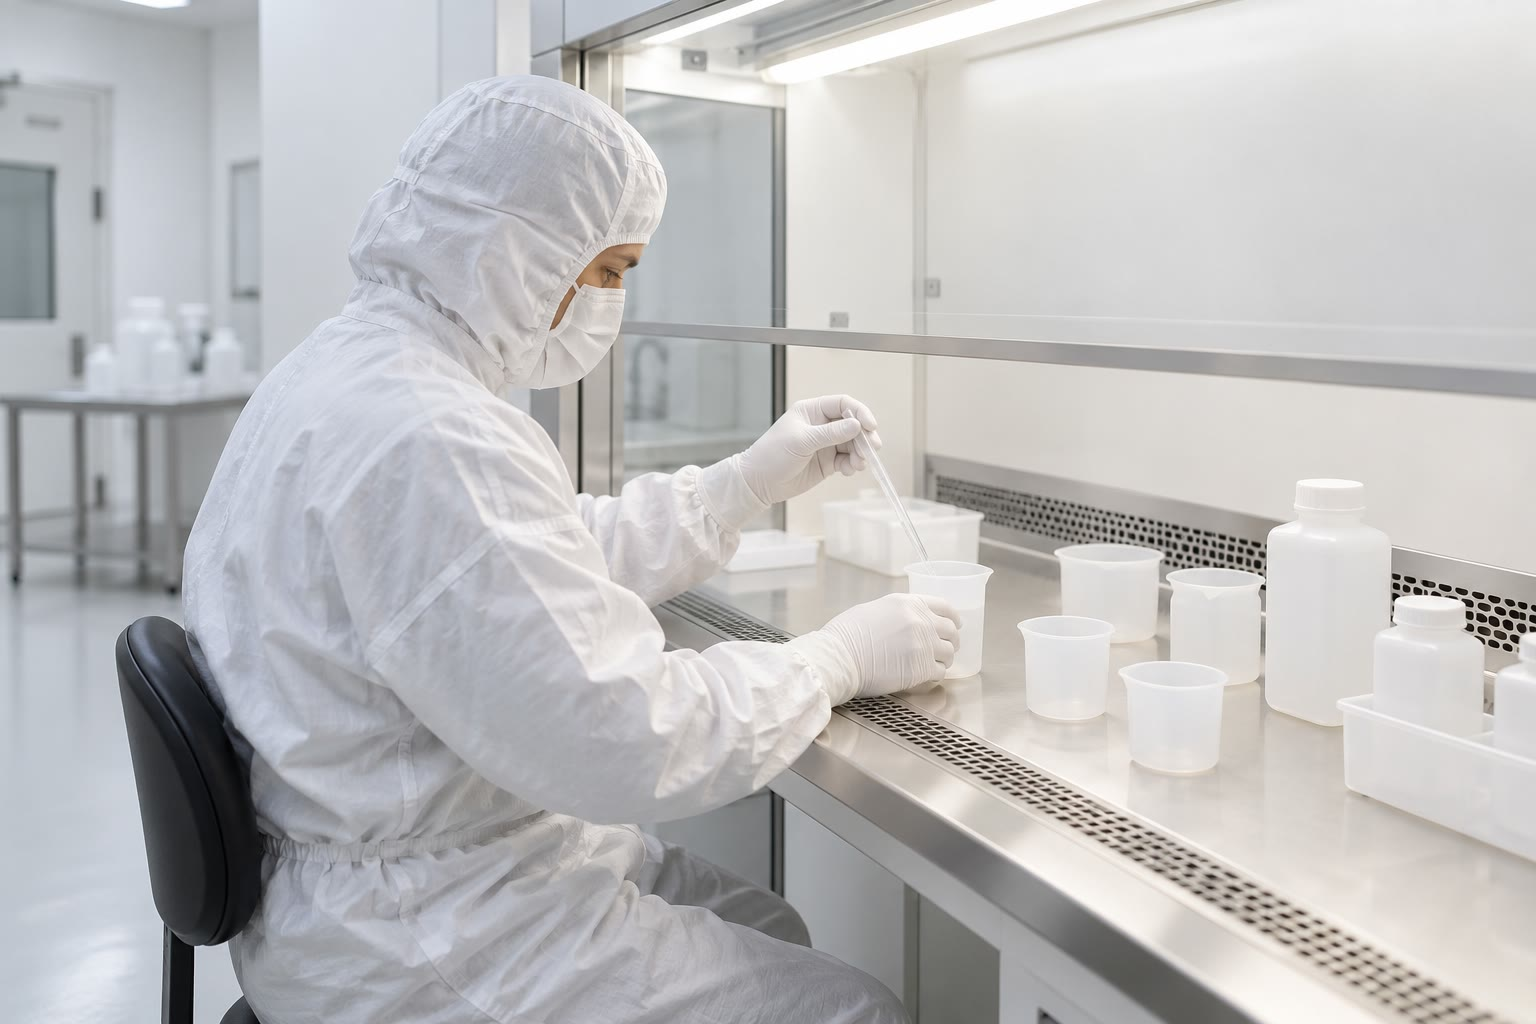
\includegraphics[width=\linewidth]{images/book4/ai/b2-clean-lab.jpg}

\smallskip
{\footnotesize किसी भू-रसायन स्वच्छ प्रयोगशाला की स्तरीय-प्रवाह बेंच पर स्वच्छ-कक्ष पोशाक में
एक कार्यकर्ता (AI से बनाया गया चित्रण)।\par}
\end{minipage}
\end{inthelab}
% ledger: usgs:bhvo2-trace, usgs:bhvo2-origin

\section{अभ्यास}

\begin{exercise}[$\star$]\label{exo:b2:elements-in-the-earth:1}
बेसाल्ट BHVO-2 में द्रव्यमान से 0.5130 प्रतिशत \ce{K2O} और 2.731 प्रतिशत \ce{TiO2}
है। परमाणु द्रव्यमान K 39.10, Ti 47.87 और O 16.00 लेकर, उसमें
पोटैशियम और टाइटेनियम की मात्राएँ ppm में परिकलित कीजिए।
\end{exercise}

\begin{exercise}[$\star$]\label{exo:b2:elements-in-the-earth:2}
\omterm{def:b2:elements-in-the-earth:bse}{समग्र सिलिकेट पृथ्वी} में, अनुपात $(X/\mathrm{Mg})$ को CI अनुपातों से भाग देने पर
ऐलुमिनियम के लिए 1.16, सोडियम के लिए 0.22, निकल के लिए 0.077 और
इरिडियम के लिए 0.0029 आते हैं। इन तत्त्वों के \omterm{def:b2:planet-formation-meteorites:condensation}{संघनन तापमान} 1653, 958, 1353
और \qty{1603}{K} हैं। हर तत्त्व का गोल्डश्मिट वर्ग बताइए और हर
न्यूनता की व्याख्या कीजिए।
\end{exercise}

\begin{exercise}[$\star$]\label{exo:b2:elements-in-the-earth:3}
ऊपरी महाद्वीपीय भूपर्पटी में \qty{31}{ppm} लैंथेनम और \qty{2.0}{ppm}
इटर्बियम है; \omterm{def:b2:elements-in-the-earth:ci}{CI कॉन्ड्राइटों} में 0.232 और \qty{0.163}{ppm}। \omterm{def:b2:planet-formation-meteorites:chondrule}{कॉन्ड्राइट} से
प्रसामान्यीकृत मान और $(\mathrm{La}/\mathrm{Yb})_N$ परिकलित कीजिए। यह
अनुपात भूपर्पटी के बारे में क्या बताता है?
\end{exercise}

\begin{exercise}[$\star$]\label{exo:b2:elements-in-the-earth:4}
ऊपरी महाद्वीपीय भूपर्पटी में 4.7, 1.0 और \qty{4.0}{ppm} सैमेरियम,
यूरोपियम और गैडोलिनियम है; \omterm{def:b2:elements-in-the-earth:ci}{CI कॉन्ड्राइटों} में 0.145, 0.0546 और \qty{0.198}{ppm}।
$\mathrm{Eu}/\mathrm{Eu}^*$ परिकलित कीजिए। कौन-सा खनिज परिणाम की व्याख्या करता है?
\end{exercise}

\begin{exercise}[$\star\star$]\label{exo:b2:elements-in-the-earth:5}
एक गार्नेट पाइरॉक्सिनाइट 65 प्रतिशत क्लाइनोपाइरॉक्सीन, 18 प्रतिशत गार्नेट और
17 प्रतिशत ओलिवीन, ऑर्थोपाइरॉक्सीन तथा स्पिनेल से बना है। लैंथेनम के विभाजन गुणांक
0.058, 0.001 और 0.001 हैं, ल्यूटेशियम के 0.53, 5.8 और 0.18।
समग्र गुणांक परिकलित कीजिए। चट्टान में कौन-सा तत्त्व संगत है? चट्टान के
ल्यूटेशियम का अधिकांश भाग कौन-सा खनिज धारण करता है?
\end{exercise}

\begin{exercise}[$\star\star$]\label{exo:b2:elements-in-the-earth:6}
\omterm{def:b2:elements-in-the-earth:bse}{समग्र सिलिकेट पृथ्वी} में 22.8 प्रतिशत मैग्नीशियम, \qty{2670}{ppm}
सोडियम और \qty{1960}{ppm} निकल है; \omterm{def:b2:elements-in-the-earth:ci}{CI कॉन्ड्राइटों} में 9.587 प्रतिशत,
\qty{5010}{ppm} और \qty{10640}{ppm}। सोडियम और निकल के लिए CI के सापेक्ष
Mg से प्रसामान्यीकृत अनुपात परिकलित कीजिए। दोनों तत्त्व \qty{1000}{K} के निकट या उससे ऊपर संघनित होते हैं;
निकल अधिक न्यून क्यों है?
\end{exercise}

\begin{exercise}[$\star\star$]\label{exo:b2:elements-in-the-earth:7}
माध्य MORB के संघटन वाले गलित से, जिसमें
\qty{5.21}{ppm} लैंथेनम और \qty{0.53}{ppm} ल्यूटेशियम है, एक क्लाइनोपाइरॉक्सीन क्रिस्टलित होता है। उसके विभाजन
गुणांक लैंथेनम के लिए 0.058 और ल्यूटेशियम के लिए 0.53 हैं। उसमें
लैंथेनम और ल्यूटेशियम की मात्राएँ, और क्रिस्टल में $(\mathrm{La}/\mathrm{Lu})_N$ का
गलित में उसके मान से अनुपात परिकलित कीजिए (CI: La 0.232, Lu \qty{0.0237}{ppm})।
\end{exercise}

\begin{exercise}[$\star\star$]\label{exo:b2:elements-in-the-earth:8}
\omterm{def:b2:elements-in-the-earth:bse}{आद्य प्रावार} (Nb \qty{0.658}{ppm}, La \qty{0.648}{ppm}) से प्रसामान्यीकृत करके,
ऊपरी महाद्वीपीय भूपर्पटी (Nb 12,
La \qty{31}{ppm}), हवाई के बेसाल्ट (18.10, \qty{15.20}{ppm}) और माध्य MORB
(5.24, \qty{5.21}{ppm}) के लिए $(\mathrm{Nb}/\mathrm{La})_N$ परिकलित कीजिए। इनमें से किसमें क्षेपण क्षेत्रों का चिह्न है?
\end{exercise}

\begin{exercise}[$\star\star$]\label{exo:b2:elements-in-the-earth:9}
पोटैशियम और यूरेनियम दोनों अत्यधिक असंगत हैं। द्रव्यमान-अनुपात K/U परिकलित कीजिए:
\omterm{def:b2:elements-in-the-earth:bse}{आद्य प्रावार} में (K \qty{240}{ppm}, U \qty{0.0203}{ppm}), माध्य MORB में
(\qty{0.160}{\percent} \ce{K2O}, U \qty{0.119}{ppm}) और ऊपरी महाद्वीपीय
भूपर्पटी में (\qty{2.80}{\percent} \ce{K2O}, U \qty{2.7}{ppm}), द्रव्यमान से
$\mathrm{K}/\ce{K2O} = 0.830$ लेकर। अनुपात के लगभग स्थिर रहने का क्या
अर्थ है, और किसी ग्रह के पोटैशियम का अनुमान लगाने के लिए K/U क्यों उपयोगी है?
\end{exercise}

\begin{exercise}[$\star\star\star$]\label{exo:b2:elements-in-the-earth:10}
गलित की एक छोटी मात्रा अभ्यास 5 के गार्नेट पाइरॉक्सिनाइट के साथ साम्यावस्था में
है। दिखाइए कि दो तत्त्वों के लिए अनुपात
$(C_1/C_2)_{\mathrm{melt}}/(C_1/C_2)_{\mathrm{rock}}$
$\bar D_2/\bar D_1$ के बराबर है। लैंथेनम और ल्यूटेशियम के लिए इसे परिकलित कीजिए, और समझाइए कि
गार्नेट-युक्त प्रावार के गलितों के दुर्लभ मृदा प्रतिरूप तीव्र ढलान वाले क्यों होते हैं।
\end{exercise}

\begin{exercise}[$\star\star\star$]\label{exo:b2:elements-in-the-earth:11}
एक माध्य MORB (Th \qty{0.404}{ppm}, Nb \qty{5.24}{ppm}) ऊपरी
महाद्वीपीय भूपर्पटी (Th \qty{10.5}{ppm}, Nb \qty{12}{ppm}) को आत्मसात करता है: भूपर्पटी का द्रव्यमान-अंश $f$
बेसाल्ट के $1-f$ के साथ मिलता है। दिखाइए कि मिश्रण की सांद्रताएँ
$f$ में रैखिक हैं पर उसका अनुपात Th/Nb नहीं। वह $f$ ज्ञात कीजिए जिसके लिए Th/Nb
0.2 तक पहुँचता है, और $f = 0.1$ के लिए अनुपात।
\end{exercise}

\begin{exercise}[$\star\star\star$]\label{exo:b2:elements-in-the-earth:12}
जल, कार्बन या ऐसे धात्विक क्रोड को हटाने से, जिसमें न ऐलुमिनियम हो न
मैग्नीशियम, शेष का अनुपात Al/Mg नहीं बदलता: इसे दिखाइए। \omterm{def:b2:elements-in-the-earth:bse}{समग्र
सिलिकेट पृथ्वी} में $(\mathrm{Al}/\mathrm{Mg})$ CI मान का 1.16 गुना है। यदि
पृथ्वी ने अपना सारा ऐलुमिनियम रखा, तो उसके कॉन्ड्राइटी मैग्नीशियम का कितना अंश
सिलिकेट पृथ्वी से गायब है? सिलिकॉन के Mg से प्रसामान्यीकृत अनुपात,
0.83, के साथ उसी मान्यता पर उसके कॉन्ड्राइटी सिलिकॉन का कितना अंश
गायब होता?
\end{exercise}

\section{समस्या: एक कॉन्ड्राइट से क्रोड को तौलना}

\begin{problem}[{सप्ताहांत समस्या --- CI कॉन्ड्राइटों, प्रावार और क्रोड से समग्र पृथ्वी का
पुनर्निर्माण, और क्रोड को तौलना}]
\label{pb:b2:elements-in-the-earth:1}
एक ग्रहीय भू-रसायनविद् पृथ्वी के क्रोड को भूकंपविज्ञान के बिना, केवल
रसायन से तौलना चाहती है। वह \omterm{def:b2:elements-in-the-earth:ci}{CI कॉन्ड्राइटों} को आरंभिक सामग्री के रूप में लेती है (Mg
\qty{95870}{ppm}, Al 8500, Si \num{106500}, Fe \num{182800}, Ni
\qty{10640}{ppm}), सिलिकेट पृथ्वी के लिए \omterm{def:b2:elements-in-the-earth:bse}{आद्य प्रावार} (MgO 37.8, FeO
8.05, NiO 0.25 प्रतिशत; Mg 22.8, Si 21.0 प्रतिशत), और 85.5
प्रतिशत Fe, 5.2 प्रतिशत Ni और 6.0 प्रतिशत Si का एक मॉडल क्रोड। परमाणु द्रव्यमान: Mg 24.31,
Si 28.09, Fe 55.85, Ni 58.69, O 16.00। पृथ्वी का द्रव्यमान
\qty{5.972e24}{kg}।

\medskip\noindent\textbf{भाग I --- कॉन्ड्राइटी आरंभ-बिंदु।}
\begin{enumerate}
\item \omterm{def:b2:elements-in-the-earth:ci}{CI कॉन्ड्राइटों} के द्रव्यमान-अनुपात Fe/Mg, Ni/Mg, Si/Mg और Al/Mg परिकलित कीजिए।
\item Fe/Si को परमाणु-अनुपात में बदलिए। सौर प्रकाशमंडल की स्पेक्ट्रमिकी
प्रति सिलिकॉन परमाणु 0.81 लोहे के परमाणु देती है: क्या तुलना सार्थक है?
\item \omterm{def:b2:elements-in-the-earth:ci}{CI कॉन्ड्राइटों} में 2.1 प्रतिशत हाइड्रोजन और 3.5 प्रतिशत कार्बन है, जो
जलयुक्त खनिजों और कार्बनिक यौगिकों में बँधे हैं जिन्हें पृथ्वी ने नहीं रखा। प्रश्न 1 के
अनुपातों को इस हानि के लिए संशोधित करने की आवश्यकता क्यों नहीं है?
\item क्रोड की समस्या के लिए मैग्नीशियम उपयुक्त संदर्भ तत्त्व क्यों है, और
लोहा यह काम क्यों नहीं कर सकता?
\item निकल, मैग्नीशियम, लोहा और सिलिकॉन एक-दूसरे के \qty{50}{K} के भीतर संघनित होते हैं
(1353, 1336, 1334 और \qty{1310}{K})। यह इस
मान्यता का समर्थन क्यों करता है कि समग्र पृथ्वी ने उनके कॉन्ड्राइटी अनुपात रखे? प्रश्न 1 का कौन-सा अनुपात
इस समूह से हटता है, और अध्याय उसके बारे में क्या कहता है?
\end{enumerate}

\noindent\textbf{भाग II --- सिलिकेट पृथ्वी।}
\begin{enumerate}[resume]
\item \omterm{def:b2:elements-in-the-earth:bse}{आद्य प्रावार} के FeO और NiO को Fe और Ni में बदलिए।
\item सिलिकेट पृथ्वी में Fe/Mg और Ni/Mg परिकलित कीजिए।
\item स्थिर मैग्नीशियम पर, कॉन्ड्राइटी Fe और Ni का कितना अंश सिलिकेट
पृथ्वी से गायब है?
\item इरिडियम के लिए यही परिकलन (\omterm{def:b2:elements-in-the-earth:bse}{आद्य प्रावार} \qty{3.2}{ppb}, CI
\qty{0.470}{ppm}) 99.7 प्रतिशत का गायब अंश देता है। यह निकल की तुलना में
बड़ा क्यों है, और निकल का लोहे की तुलना में क्यों?
\item सिलिकेट पृथ्वी में लोहा कहाँ है, और वह सारा का सारा
क्रोड में क्यों नहीं गया?
\end{enumerate}

\noindent\textbf{भाग III --- क्रोड को तौलना।}
\begin{enumerate}[resume]
\item क्रोड के द्रव्यमान-अंश $x$ के साथ पृथ्वी का लौह-संतुलन लिखिए, और
\cref{prop:b2:elements-in-the-earth:core} व्युत्पन्न कीजिए।
\item लोहे से $y = x/(1-x)$ और $x$ परिकलित कीजिए।
\item यही निकल से कीजिए।
\item दोनों अनुमान ठीक-ठीक मेल नहीं खाते। उन्हें न्यूनतम वर्गों से मिलाइए:
$\sum (a_iy - b_i)^2$ को न्यूनतम कीजिए, जहाँ $a_i y = b_i$ प्रश्न 12 और 13 के
दो समीकरण हैं, और सर्वोत्तम $y$ और $x$ बताइए।
\item न्यूनतम-वर्ग मान लोहे वाले अनुमान के इतने निकट क्यों है?
\item दोनों समीकरणों से क्रोड का वह Fe/Ni अनुपात परिकलित कीजिए जो
दोनों को ठीक-ठीक सत्य बना दे। मॉडल क्रोड से तुलना कीजिए।
\item क्रोड का द्रव्यमान बताइए।
\end{enumerate}

\noindent\textbf{भाग IV --- जाँचें और परिणाम।}
\begin{enumerate}[resume]
\item भूकंपविज्ञान पृथ्वी के द्रव्यमान का 32.5 प्रतिशत क्रोड देता है। रासायनिक अनुमान
कितने प्रतिशत भिन्न है?
\item 32.5 प्रतिशत के क्रोड के साथ, लौह-संतुलन पूरा करने के लिए क्रोड में कितना लोहा
होना चाहिए? क्या यह ऐसे क्रोड से संगत है जिसका 10 प्रतिशत हल्के
तत्त्व हैं?
\item मॉडल क्रोड में Fe और Ni के अतिरिक्त अन्य तत्त्वों का 9.3 प्रतिशत है। कौन-से
हल्के तत्त्व उम्मीदवार हैं, और अध्याय में कौन-सा साक्ष्य सिलिकॉन का समर्थन करता है?
\item प्रश्न 14 के $y$ के साथ, क्रोड की वह सिलिकॉन-मात्रा परिकलित कीजिए जो
समग्र पृथ्वी के Si/Mg को कॉन्ड्राइटी बना दे।
\item मॉडल के 6 प्रतिशत से तुलना कीजिए। पिछले
अध्याय के आधार पर एक कारण सुझाइए कि कुछ सिलिकॉन पूरी पृथ्वी से ही क्यों गायब हो सकता है।
\item मॉडल क्रोड में \qty{0.5}{ppm} सोना है, \omterm{def:b2:elements-in-the-earth:bse}{आद्य प्रावार} में
\qty{1}{ppb}। 32.5 प्रतिशत के क्रोड के साथ, पृथ्वी के सोने का कितना अंश
क्रोड में है?
\item केवल रसायन से प्राप्त पृथ्वी का क्रोड द्रव्यमान-अंश बताइए,
जो इस समस्या की मुख्य संख्या है।
\end{enumerate}
\end{problem}
% ledger: lodders:ci-table, lodders:ci-h-photo, ms95:pm-oxides, ms95:pm-trace, mcd03:core, earth:mass, badro:core, lodders:tc-table
